\documentclass[a4paper,11pt]{report}
\usepackage{chuan_math_gkt}
\usetikzlibrary{angles,quotes,intersections,patterns,decorations.pathreplacing}
\chuanexamsetup

\begin{document}
\examfontsize

\examsecret{绝密$\bigstar$启用前}

\examtitle{2024年普通高等学校招生全国统一考试（新课标I卷）}{数\quad 学}

\noticetitle
\begin{examnotice}
\item 答卷前，考生务必将自己的姓名、准考证号填写在答题卡上. 
\item 回答选择题时，选出每小题的答案后，用铅笔把答题卡上对应题目的答案标号涂黑. 如需改动，用橡皮擦干净后，再选涂其他答案标号. 回答非选择题时，将答案写在答题卡上. 写在本试卷上无效. 
\item 考试结束后，将本试卷和答题卡一并交回. 
\end{examnotice}

\examsection{一、选择题：本题共8小题，每小题5分，共40分. 在每小题给出的四个选项中，只有一个选项是正确的. 请把正确的选项填涂在答题卡相应的位置上. }
\begin{examquestions}
\item 已知集合 $A=\{x\mid -5<x^3<5\}$，$B=\{-3,-1,0,2,3\}$，则 $A\cap B=$
\fourchoices{$\{-1,0\}$}{$\{2,3\}$}{$\{-3,-1,0\}$}{$\{-1,0,2\}$}
\item 若 $\dfrac{z}{z-1}=1+\mathrm{i}$，则 $z=$
\fourchoices{$-1-\mathrm{i}$}{$-1+\mathrm{i}$}{$1-\mathrm{i}$}{$1+\mathrm{i}$}
\item 已知向量 $\vec a=(0,1),\vec b=(2,x)$，若 $\vec b\perp(\vec b-4\vec a)$，则 $x=$
\fourchoices{$-2$}{$-1$}{$1$}{$2$}
\item 已知 $\cos(\alpha+\beta)=m,\tan\alpha\tan\beta=2$，则 $\cos(\alpha-\beta)=$
\fourchoices{$-3m$}{\tallchoice{$-\dfrac m3$}}{\tallchoice{$\dfrac m3$}}{$3m$}
\item 已知圆柱和圆锥底面半径相等，侧面积相等，且它们的高均为 $\sqrt3$，则圆锥的体积为
\fourchoices{$2\sqrt3\pi$}{$3\sqrt3\pi$}{$6\sqrt3\pi$}{$9\sqrt3\pi$}
\item 已知函数 $f(x)=$\linsys{-x^2-2ax-a,x<0,\\e^x+\ln(x+1),x\geq0} 在 $\mathbb R$ 上单调递增，则 $a$ 取值的范围是
\fourchoices{$(-\infty,0]$}{$[-1,0]$}{$[-1,1]$}{$[0,+\infty)$}
\item 当 $x\in[0,2\pi]$ 时，曲线 $y=\sin x$ 与 $y=2\sin\left(3x-\dfrac\pi6\right)$ 的交点个数为
\fourchoices{$3$}{$4$}{$6$}{$8$}
\item 已知函数 $f(x)$ 的定义域为 $\mathbb R$，$f(x)>f(x-1)+f(x-2)$，且当 $x<3$ 时 $f(x)=x$，则下列结论中一定正确的是
\twochoices{$f(10)>100$}{$f(20)>1000$}{$f(10)<1000$}{$f(20)<10000$}
\end{examquestions}
\examsection{二、选择题：本题共3小题，每小题6分，共18分. 在每小题给出的选项中，有多项符合题目要求. 全部选对得6分，部分选对的得部分分，有选错的得0分. }
\begin{examquestions}[start=9]
\item 为了解推动出口后的亩收入（单位：万元）情况，从该种植区抽取样本，得到推动出口后亩收入的样本均值 $\overline x=2.1$，样本方差 $s^2=0.01$，已知该种植区以往的亩收入 $X$ 服从正态分布 $N(1.8,0.1^2)$，假设推动出口后的亩收入 $Y$ 服从正态分布 $N(\overline x,s^2)$，则（若随机变量 $Z$ 服从正态分布 $N(\mu,\sigma^2)$，$P(Z<\mu+\sigma)\approx0.8413$）
\twochoices{$P(X>2)>0.2$}{$P(X>2)<0.5$}{$P(Y>2)>0.5$}{$P(Y>2)<0.8$}
\item 设函数 $f(x)=(x-1)^2(x-4)$，则
\twochoices{$x=3$ 是 $f(x)$ 的极小值点}{当 $0<x<1$ 时，$f(x)<f(x^2)$}{当 $1<x<2$ 时，$-4<f(2x-1)<0$}{当 $-1<x<0$ 时，$f(2-x)>f(x)$}
\item 造型 $\infty$ 可以做成美丽的丝带，将其看作图中曲线 $C$ 的一部分. 已知 $C$ 过坐标原点 $O$，且 $C$ 上的点满足横坐标大于 $-2$，到点 $F(2,0)$ 的距离与到定直线 $x=a(a<0)$ 的距离之积为4，则

\noindent\begin{minipage}[t]{0.64\linewidth}
\onechoices{$a=-2$}{点 $(2\sqrt2,0)$ 在 $C$ 上}{$C$ 在第一象限的点的纵坐标的最大值为1}{当点 $(x_0,y_0)$ 在 $C$ 上时，$y_0\leq\dfrac4{x_0+2}$}
\end{minipage}\hfill
\begin{minipage}[t]{0.30\linewidth}
\vspace{-1.6em}
\centering
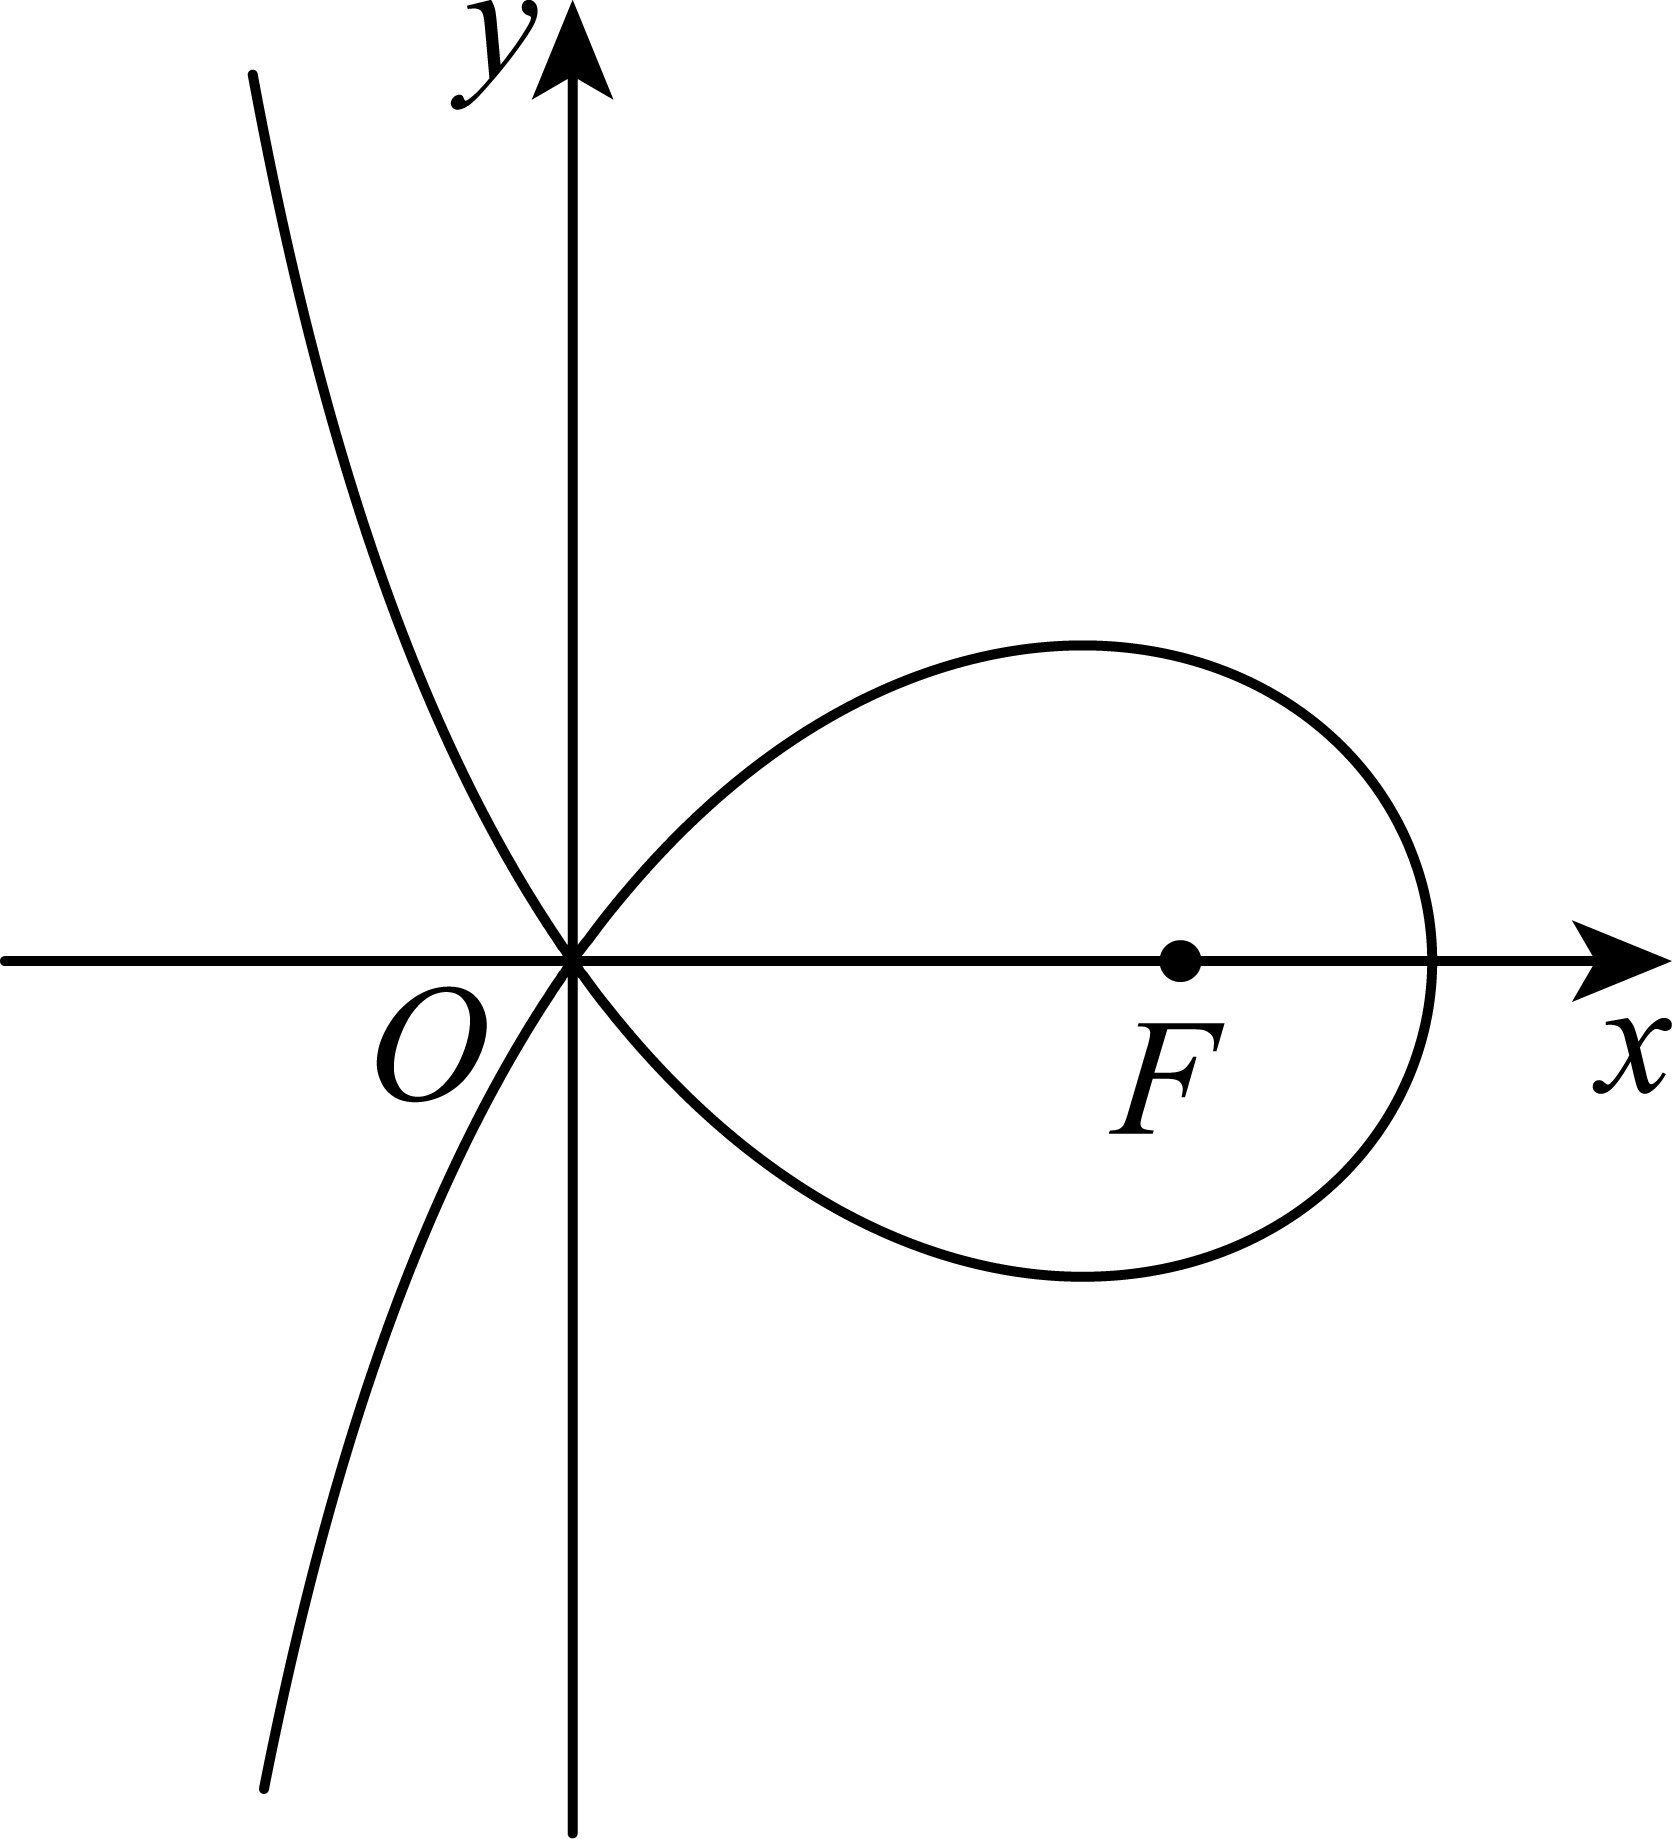
\includegraphics[width=\linewidth]{figures/2024_xgk1_q11.png}
\end{minipage}\end{examquestions}
\examsection{三、填空题：本题共3小题，每小题5分，共15分. }
\begin{examquestions}[start=12]
\item 设双曲线 $C:\dfrac{x^2}{a^2}-\dfrac{y^2}{b^2}=1(a>0,b>0)$ 的左右焦点分别为 $F_1,F_2$，过 $F_2$ 作平行于 $y$ 轴的直线交 $C$ 于 $A,B$ 两点，若 $|F_1A|=13,|AB|=10$，则 $C$ 的离心率为\blank. 
\item 若曲线 $y=e^x+x$ 在点 $(0,1)$ 处的切线也是曲线 $y=\ln(x+1)+a$ 的切线，则 $a=\blank$. 
\newpage
\item 甲、乙两人各有四张卡片，每张卡片上标有一个数字，甲的卡片上分别标有数字1，3，5，7，乙的卡片上分别标有数字2，4，6，8，两人进行四轮比赛，在每轮比赛中，两人各自从自己持有的卡片中随机选一张，并比较所选卡片上数字的大小，数字大的人得1分，数字小的人得0分，然后各自弃置此轮所选的卡片（弃置的卡片在此后的轮次中不能使用）. 则四轮比赛后，甲的总得分不小于2的概率为\blank. 
\end{examquestions}
\examsection{四、解答题：本题共5小题，共77分. 解答应写出文字说明、证明过程或演算步骤. }
\begin{examanswers}[start=15]
\item（13分）

记 $\triangle ABC$ 内角 $A,B,C$ 的对边分别为 $a,b,c$，已知 $\sin C=\sqrt2\cos B$，$a^2+b^2-c^2=\sqrt2ab$. 

（1）求 $B$；

（2）若 $\triangle ABC$ 的面积为 $3+\sqrt3$，求 $c$. 
\item（15分）

已知 $A(0,3)$ 和 $P\left(3,\dfrac32\right)$ 为椭圆 $C:\dfrac{x^2}{a^2}+\dfrac{y^2}{b^2}=1(a>b>0)$ 上两点. 

（1）求 $C$ 的离心率；

（2）若过 $P$ 的直线 $l$ 交 $C$ 于另一点 $B$，且 $\triangle ABP$ 的面积为9，求 $l$ 的方程. 
\item（15分）

如图，四棱锥 $P-ABCD$ 中，$PA\perp$ 底面 $ABCD$，$PA=AC=2$，$BC=1$，$AB=\sqrt3$. 

\noindent\begin{minipage}[t]{0.64\linewidth}
    
（1）若 $AD\perp PB$，证明：$AD\parallel$ 平面 $PBC$；

（2）若 $AD\perp DC$，且二面角 $A-CP-D$ 的正弦值为 $\dfrac{\sqrt{42}}7$，求 $AD$. 
\end{minipage}\hfill
\begin{minipage}[t]{0.22\linewidth}
\vspace{-0.6em}
\centering
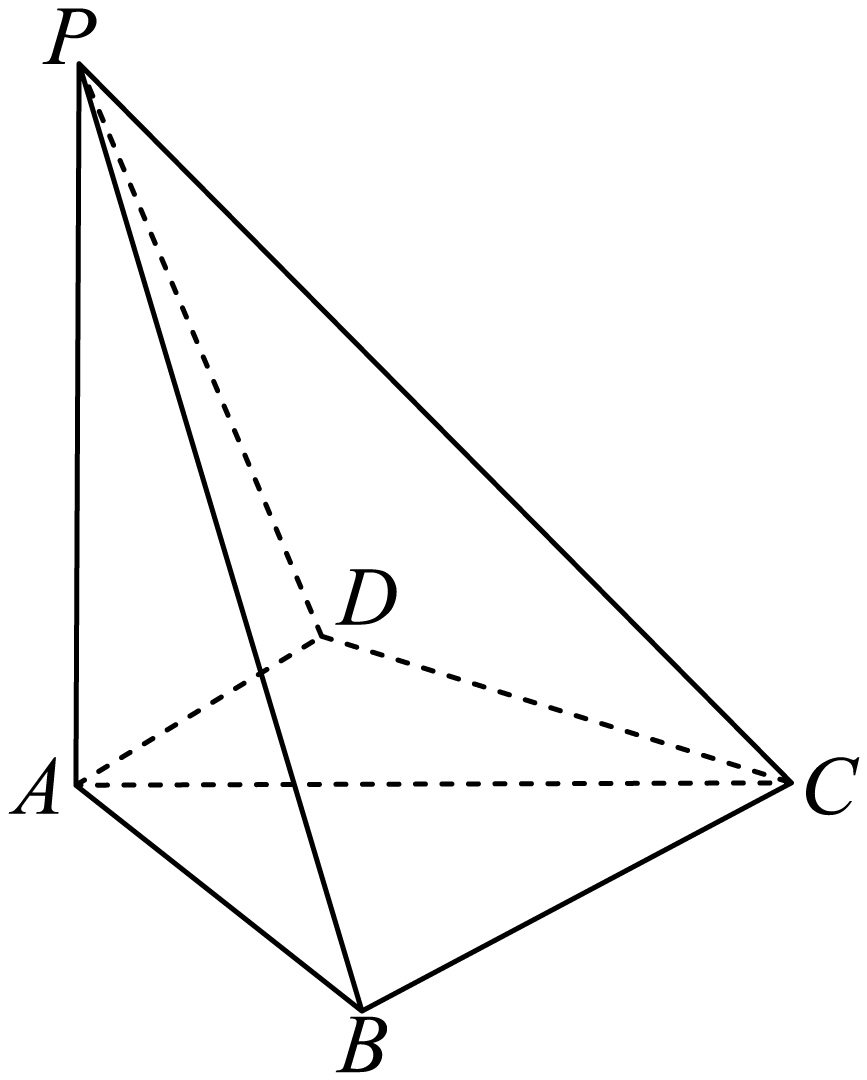
\includegraphics[width=\linewidth]{figures/2024_xgk1_q17.png}
\end{minipage}
\item（17分）

已知函数 $f(x)=\ln\dfrac{x}{2-x}+ax+b(x-1)^3$. 

（1）若 $b=0$，且 $f'(x)\geq0$，求 $a$ 的最小值；

（2）证明：曲线 $y=f(x)$ 是中心对称图形；

（3）若 $f(x)>-2$ 当且仅当 $1<x<2$，求 $b$ 的取值范围. 
\item（17分）

设 $m$ 为正整数，数列 $a_1,a_2,\cdots,a_{4m+2}$ 是公差不为0的等差数列，若从中删去两项 $a_i$ 和 $a_j(i<j)$ 后剩余的 $4m$ 项可被平均分为 $m$ 组，且每组的4个数都能构成等差数列，则称数列 $a_1,a_2,\cdots,a_{4m+2}$ 是 $(i,j)$-可分数列. 

（1）写出所有 $(i,j)$，$1\leq i<j\leq6$，使数列 $a_1,a_2,\cdots,a_6$ 是 $(i,j)$-可分数列；

（2）当 $m\geq3$ 时，证明：数列 $a_1,a_2,\cdots,a_{4m+2}$ 是 $(2,13)$-可分数列；

（3）从 $1,2,\cdots,4m+2$ 中一次任取两个数 $i$ 和 $j(i<j)$，记数列 $a_1,a_2,\cdots,a_{4m+2}$ 是 $(i,j)$-可分数列的概率为 $P_m$，证明：$P_m>\dfrac18$. 
\end{examanswers}

\end{document}
